\chapter{Ala i estabilitzadors}

Un cop estudiat el comportament de l'ala aïllada, s'ha d'estudiar el comportament del planejador complet, tenint en compte tant l'estabilitzador horitzontal com el vertical i per tant les interaccions i interferències que aixo produeix respecte l'ala aïllada. 

Per tal d'estudiar el conjunt, s'assumeix que l'estabilitzador horitzontal te un angle de torsió o twist nul. A més, s'estableix que l'estabilitzador horitzontal només produeix una resistència aerodinàmica parasita ja que presenta un angle de lliscament $\beta=0^{\circ}$ i per tant no genera sustentació ni conseqüentment resistència induïda. 

\section{Coeficients Aerodinàmics}

Primerament s'estudia el comportament calculant tant el coeficient de sustentació com el de resistència pel conjunt ala-estabilitzadors en funció de l'angle d'atac (veure Figures \ref{CLvsalpha} y \ref{CDvsalpha}).

Per una configuració de vol amb un angle d'atac de valor $\alpha=6^{\circ}$ s'obté: $C_{L} = 0.865 $ y $C_{D} = 0.0276 $

\begin{figure}[h]
	\centering
	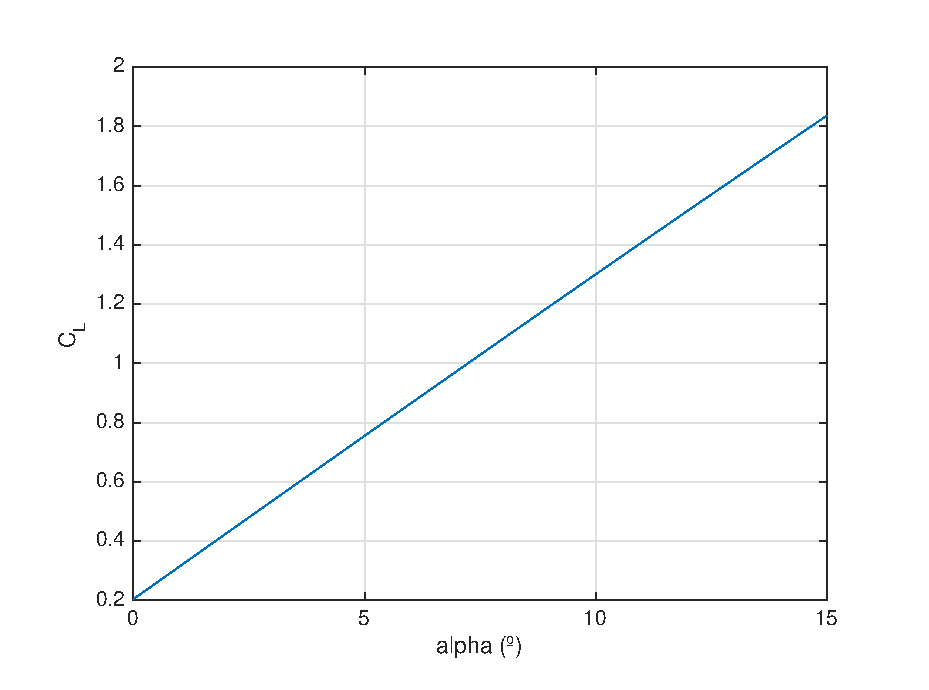
\includegraphics[width=0.9\textwidth]{./plots/CLvsalpha_4}
	\caption{Coeficient de sustentació en funció de l'angle d'atac}
	\label{CLvsalpha}
\end{figure}

\begin{figure}[h]
	\centering
	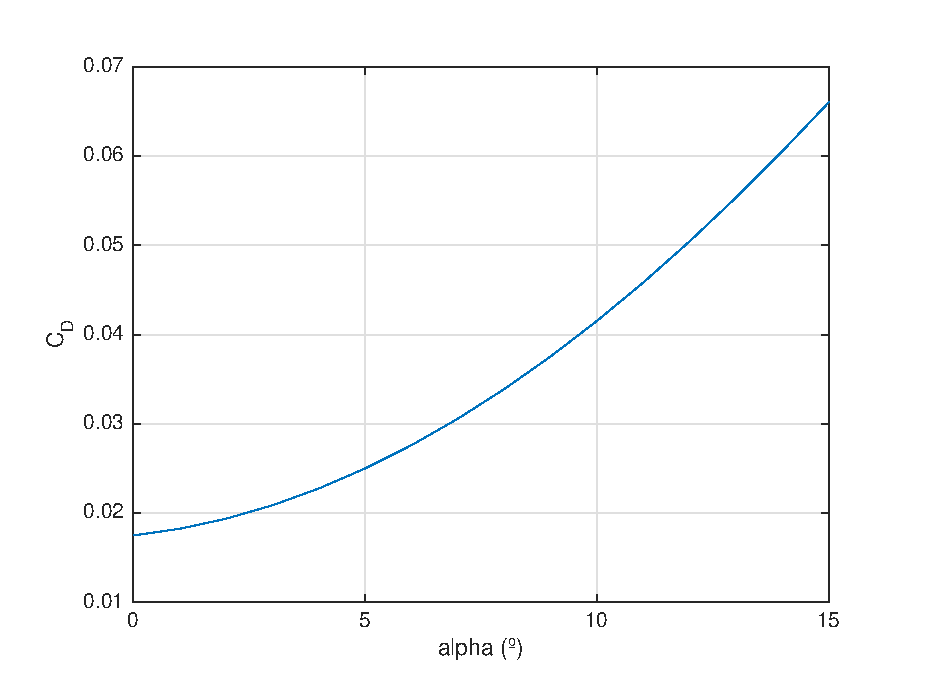
\includegraphics[width=0.9\textwidth]{./plots/CDvsalpha_4}
	\caption{Coeficient de resistència en funció de l'angle d'atac}
	\label{CDvsalpha}
\end{figure}


 
\section{Posició del centre de masses} 

Finalment, s'estudia l'estabilitat del planejador. Per fer-ho es calcula la posició del centre de masses que fa que el conjunt ala-estabilitzadors sigui longitudinalment estable. 

Per realitzar el calcul s'agafa la congiguració d'angle d'atac vista a l'apartat anterior, $\alpha=6^{\circ}$, i s'imposa que el sumatori de moments respecte el centre de masses (punt a trobar) sigui igual a zero. L'algoritme seguit per fer-ho es mostra a la Figura \ref{AlgoritmeCM}.

\begin{figure}[h]
	\centering
	\includegraphics[scale=0.5]{./plots/algoritmeCM}
	\caption{Algoritme seguit pel càlcul de la posició del centre de masses}
	\label{AlgoritmeCM}
\end{figure}

Així doncs, un cop realitzat els calculs s'obté $X_{CM} = 0.256 $ 